\chapter{Background}

A continuous surface---a surface defined by a continuous function $f(x,y,z)=0$---could be said to
consist of an infinite number of points (namely, all points in $\mathbb{R}^3$ where the equation
holds true).  In real-time computer graphics, however, we normally define surfaces (called
\textit{meshes}) using \textit{vertices} and \textit{triangles}.  This is usually also a good-enough
approximation of a continuous surface and gives a vast improvement in rendering performance
(although, it should be noted that, depending on the context, the gap is narrowing, see
\citet{chang2015}).

\fig{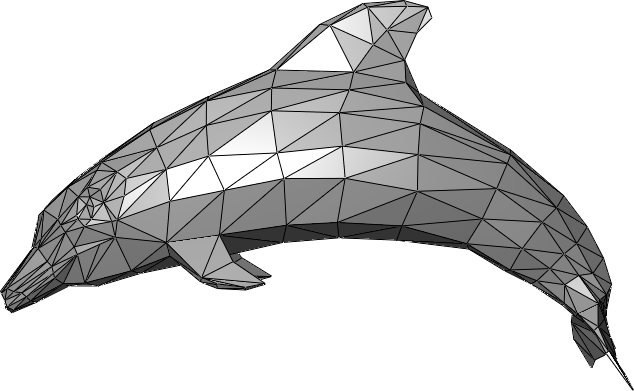
\includegraphics[width=0.5\textwidth]{dolphin-triangle-mesh}}{A dolphin triangle mesh.}

A higher density triangle mesh has more triangles in it, thus enabling it to model finer detail.
For the sake of computational efficiency, we always use the lowest feasible resolution to model the
detail required by the scene.
